\documentclass{beamer}
\usepackage{bjtu}
\usepackage{graphicx}
\graphicspath{ {./images/} {./logo/}}

% show table of contents at begin of each section
\AtBeginSection[]
{
  \begin{frame}
    \frametitle{Table of Contents}
    \setcounter{tocdepth}{1}
    \tableofcontents[currentsection]
  \end{frame}
}

%===================================================
%===================================================
\title{title}
\author{Cao Xuyang}
\date{2019.05.17}
\logo{
\includegraphics[width=1cm,height=1cm]{logo_bjtu}\hspace{1.05\textwidth}\vspace{240pt}}

%===================================================
%===================================================
\begin{document}
\frame[plain]{\titlepage}                  % title page
\begin{frame}{Table of Contents(目录)}    % table of contents frame 
    \setcounter{tocdepth}{1}        % 只显示一层目录结构
    \tableofcontents                % table of contents
\end{frame}
\begin{frame}{医学图像处理}
    \alert{哈哈}
\end{frame}{}

%==================在这下面添加内容=================
\section{Section 1}
\begin{frame}[c]{Test Frame} % 参数c表示内容垂直居中,默认是顶部对齐[t]
    这是参考文献测试\cite{Cheplygina2018NotsosupervisedAS}
    
    这是一段中文测试
    
    公式:
    \[Dice = \frac{2 |A \cap B|}{|A| + |B|}\]
\end{frame}
 
\section{Section 2}
\begin{frame}[c]{Frame Title}
    \begin{columns}
    \column{0.5\textwidth}
    This is a text in first column.
    $$E=mc^2$$
    \begin{itemize}
    \item First item
    \item Second item
    \end{itemize}
     
    \column{0.5\textwidth}
    This text will be in the second column
    and on a second tought this is a nice looking
    layout in some cases.
    \end{columns}
\end{frame}


\begin{frame}{Frame Title}

\begin{columns}
\column{0.5\textwidth}
\begin{figure}
    \centering
    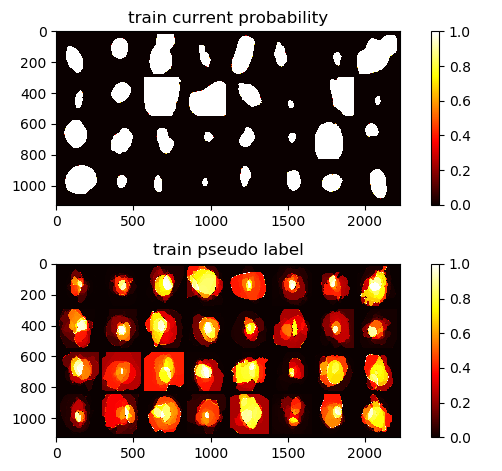
\includegraphics[width=1.\textwidth]{images/before.png}
    \caption*{Before}
\end{figure}

\column{0.5\textwidth}
\begin{figure}
    \centering
    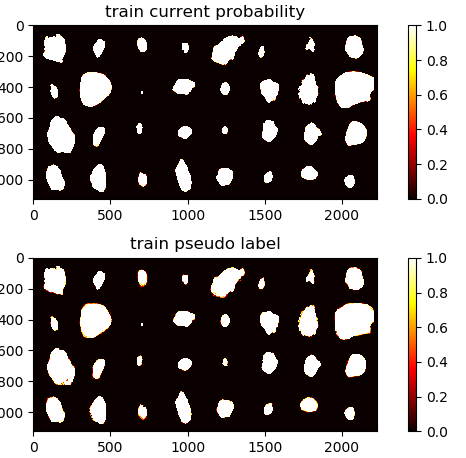
\includegraphics[width=1.\textwidth]{images/after.png}
    \caption*{After}
\end{figure}
\end{columns}
\end{frame}

\subsection{subsection 1}
%==================在这上面添加内容=================

\begin{frame}{Reference}
    \bibliographystyle{unsrt}
    \bibliography{references}
  
\end{frame}
\end{document}